\subsection{Reunión individual}\label{addReunionIndividual}

  \paragraph{}La gestión de las reuniones individuales para el usuario
  \textit{Asesor} es idéntica a la comentada para el usuario
  \textit{Administrador principal} en la sección \ref{gestionReunion},
  con la única diferencia de que solo estarán disponibles los alumnos a los que
  este usuario preste asesoría en el curso académico actual.

  \paragraph{}Desde este listado, el usuario asesor podrá añadir preguntas,
  bien oficiales o bien de reunión, a una reunión individual, además de ver las
  ya existentes. La figura \ref{capturaPantallaReunionIndividual} muestra esta
  ventana.

  \begin{figure}[!ht]
    \begin{center}
      \fbox{
      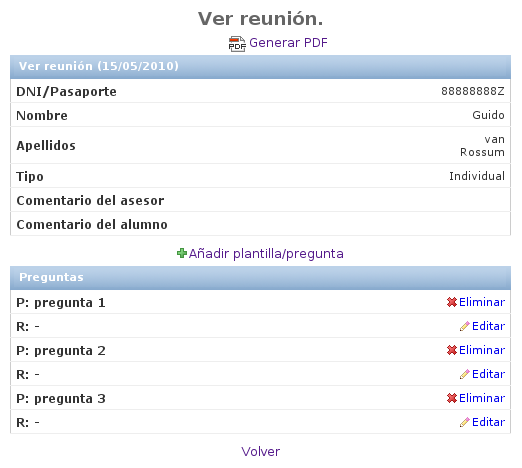
\includegraphics[scale=0.55]{4.Funcionamiento_Aplicacion/4.3.Gestion/4.3.3.Asesor/4.3.3.7.ReunionIndividual/lista_reunion.png}
      }
      \caption{Captura de pantalla del listado de una reunión individual para el usuario \textit{Asesor}.}
      \label{capturaPantallaReunionIndividual}
    \end{center}
  \end{figure}

  \paragraph{}Al pulsar en el enlace \textit{Añadir plantilla/pregunta},
  aparecerá una ventana con las plantillas y preguntas disponibles para este
  usuario. Esta ventana es la mostrada en la figura
  \ref{capturaPantallaAddPlantillaReunionInd}.

  \begin{figure}[!ht]
    \begin{center}
      \fbox{
      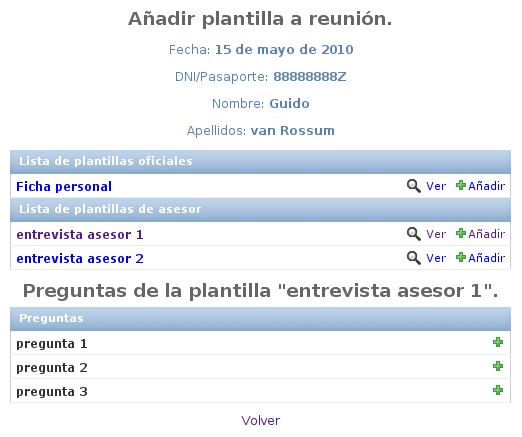
\includegraphics[scale=0.55]{4.Funcionamiento_Aplicacion/4.3.Gestion/4.3.3.Asesor/4.3.3.7.ReunionIndividual/add_plantilla.png}
      }
      \caption{Captura de pantalla del listado de plantillas y preguntas para el usuario \textit{Asesor}.}
      \label{capturaPantallaAddPlantillaReunionInd}
    \end{center}
  \end{figure}
